%%%%%%%%%%%%%%%%%%%%%%%%%%%%%%%%%%%%%%%%%%%%%%%%%%%%%%%%%%%%%
% CÁC BƯỚC THỰC HIỆN TRƯỚC KHI SOẠN BÁO CÁO
%   1. Sửa footer tại line 84
%   2. Sửa tên môn học, Mã số MH tại line 172
%   3. Sửa tiêu đề báo cáo tại line 176-179
%   4. Sửa tên GVHD tại line 189
%   5. Sửa danh sách SV thực hiện tại line 191
%%%%%%%%%%%%%%%%%%%%%%%%%%%%%%%%%%%%%%%%%%%%%%%%%%%%%%%%%%%%%


\documentclass[a4paper]{article}
\usepackage{vntex}
%\usepackage[english,vietnam]{babel}
%\usepackage[utf8]{inputenc}

%\usepackage[utf8]{inputenc}
%\usepackage[francais]{babel}
\usepackage{a4wide,amssymb,epsfig,latexsym,array,hhline,fancyhdr}
\usepackage{listings}
\usepackage{amsmath}
\usepackage{amsthm}
\usepackage{multicol,longtable,amscd}
\usepackage{diagbox}%Make diagonal lines in tables
\usepackage{booktabs}
\usepackage{alltt}
\usepackage[framemethod=tikz]{mdframed}% For highlighting paragraph backgrounds
\usepackage{caption,subcaption}
\usepackage[section]{placeins}
\usepackage{lastpage}
\usepackage[lined,boxed,commentsnumbered]{algorithm2e}
\usepackage{enumerate}
\usepackage{color}
\usepackage{graphicx}							% Standard graphics package
\usepackage{array}
\usepackage{tabularx, caption}
\usepackage{multirow}
\usepackage{multicol}
\usepackage{rotating}
\usepackage{graphics}
\usepackage{geometry}
\usepackage{setspace}
\usepackage{epsfig}
\usepackage{tikz}
\usetikzlibrary{arrows,snakes,backgrounds}
\usepackage[unicode]{hyperref}
\hypersetup{urlcolor=blue,linkcolor=black,citecolor=black,colorlinks=true}
\usepackage{float} % dành cho [H]
\usepackage{wrapfig}
\usepackage{enumitem}


%\usepackage{pstcol} 								% PSTricks with the standard color package

%\newtheorem{theorem}{{\bf Định lý}}
%\newtheorem{property}{{\bf Tính chất}}
%\newtheorem{proposition}{{\bf Mệnh đề}}
%\newtheorem{corollary}[proposition]{{\bf Hệ quả}}
%\newtheorem{lemma}[proposition]{{\bf Bổ đề}}


%\usepackage{fancyhdr}
\setlength{\headheight}{40pt}
\pagestyle{fancy}
\fancyhead{} % clear all header fields
\fancyhead[L]{
 \begin{tabular}{rl}
    \begin{picture}(25,15)(0,0)
    \put(0,-8){
\includegraphics[width=8mm, height=8mm]{Images/LogoBK.jpg}}
    %\put(0,-8){\epsfig{width=10mm,figure=hcmut.eps}}
   \end{picture}&
	%
\includegraphics[width=8mm, height=8mm]{LogoBK.jpg} & %
	\begin{tabular}{l}
		\textbf{\bf \ttfamily Trường Đại Học Bách Khoa Tp.Hồ Chí Minh}\\
%		\textbf{\bf \ttfamily Khoa Khoa Học và Kỹ Thuật Máy Tính}
	\end{tabular} 	
 \end{tabular}
}
\fancyhead[R]{
	\begin{tabular}{l}
		\tiny \bf \\
		\tiny \bf 
	\end{tabular}  }
\fancyfoot{} % clear all footer fields
\fancyfoot[L]{\scriptsize \ttfamily Báo cáo môn Mạng máy tính (CO3004), HK2, năm học 2020-2021}
\fancyfoot[R]{\scriptsize \ttfamily Trang {\thepage}/\pageref{LastPage}}
\renewcommand{\headrulewidth}{0.3pt}
\renewcommand{\footrulewidth}{0.3pt}


%%%
\setcounter{secnumdepth}{4}
\setcounter{tocdepth}{3}
\makeatletter
\newcounter {subsubsubsection}[subsubsection]
\renewcommand\thesubsubsubsection{\thesubsubsection .\@alph\c@subsubsubsection}
\newcommand\subsubsubsection{\@startsection{subsubsubsection}{4}{\z@}%
                                     {-3.25ex\@plus -1ex \@minus -.2ex}%
                                     {1.5ex \@plus .2ex}%
                                     {\normalfont\normalsize\bfseries}}
\newcommand*\l@subsubsubsection{\@dottedtocline{3}{10.0em}{4.1em}}
\newcommand*{\subsubsubsectionmark}[1]{}
\makeatother
\everymath{\color{blue}}%make in-line maths symbols blue to read/check easily

\sloppy
\captionsetup[figure]{labelfont={small,bf},textfont={small,it},belowskip=0pt,aboveskip=10pt}
%space remove between caption, figure, and text
\captionsetup[table]{labelfont={small,bf},textfont={small,it},belowskip=0pt,aboveskip=10pt}
%space remove between caption, table, and text

%\floatplacement{figure}{H}%forced here float placement automatically for figures
%\floatplacement{table}{H}%forced here float placement automatically for table
%the following settings (11 lines) are to remove white space before or after the figures and tables
%\setcounter{topnumber}{2}
%\setcounter{bottomnumber}{2}
%\setcounter{totalnumber}{4}
%\renewcommand{\topfraction}{0.85}
%\renewcommand{\bottomfraction}{0.85}
%\renewcommand{\textfraction}{0.15}
%\renewcommand{\floatpagefraction}{0.8}
%\renewcommand{\textfraction}{0.1}
\setlength{\floatsep}{5pt plus 2pt minus 2pt}
\setlength{\textfloatsep}{5pt plus 2pt minus 2pt}
\setlength{\intextsep}{10pt plus 2pt minus 2pt}


\definecolor{dkgreen}{rgb}{0,0.6,0}
\definecolor{gray}{rgb}{0.5,0.5,0.5}
\definecolor{mauve}{rgb}{0.58,0,0.82}
\lstset{frame=tb,
  language=Matlab,
  aboveskip=3mm,
  belowskip=3mm,
  showstringspaces=false,
  columns=flexible,
  basicstyle={\small\ttfamily},
  numbers=none,
  numberstyle=\tiny\color{gray},
  keywordstyle=\color{blue},
  commentstyle=\color{dkgreen},
  stringstyle=\color{mauve},
  breaklines=true,
  breakatwhitespace=true,
  tabsize=3
}

%New colors defined below
\definecolor{codegreen}{rgb}{0,0.6,0}
\definecolor{codegray}{rgb}{0.5,0.5,0.5}
\definecolor{codepurple}{rgb}{0.58,0,0.82}
\definecolor{backcolour}{rgb}{0.95,0.95,0.92}

%Code listing style named "mystyle"
\lstdefinestyle{mystyle}{
  backgroundcolor=\color{backcolour},   commentstyle=\color{codegreen},
  keywordstyle=\color{magenta},
  numberstyle=\tiny\color{codegray},
  stringstyle=\color{codepurple},
  basicstyle=\ttfamily\footnotesize,
  breakatwhitespace=false,         
  breaklines=true,                 
  captionpos=b,                    
  keepspaces=true,                 
  numbers=left,                    
  numbersep=5pt,                  
  showspaces=false,                
  showstringspaces=false,
  showtabs=false,                  
  tabsize=2
}

%"mystyle" code listing set
\lstset{style=mystyle}

\begin{document}
%%%%%%%%%%%%%%%%%%%%%%%%%%%%%%%%%%%%%%%%%%%%%%%%%%%%%%%%%
%                   FIRST PAGE                          %
%%%%%%%%%%%%%%%%%%%%%%%%%%%%%%%%%%%%%%%%%%%%%%%%%%%%%%%%%

\begin{titlepage}
\begin{center}
ĐẠI HỌC QUỐC GIA THÀNH PHỐ HỒ CHÍ MINH \\
TRƯỜNG ĐẠI HỌC BÁCH KHOA \\
%KHOA KHOA HỌC - KỸ THUẬT MÁY TÍNH 
\end{center}

\vspace{1cm}

\begin{figure}[H]
\begin{center}

\includegraphics[width=3cm]{Images/LogoBK.jpg}
\end{center}
\end{figure}

\vspace{1cm}


\begin{center}
\begin{tabular}{c}
\multicolumn{1}{c}{\textbf{{\Large MẠNG MÁY TÍNH (CO3004)}}}\\
~~\\
\hline
\\
\multicolumn{1}{l}{\textbf{{\Large Bài tập lớn 2}}}\\
\\
\textbf{{\Huge Thiết kế mạng máy tính}} \\
\textbf{{\Huge cho công ty IT HK2}} \\
\\
\hline
\end{tabular}
\end{center}

\vspace{1.5cm}

\begin{table}[h]
\begin{tabular}{rrll}
\hspace{4 cm} & GVHD: & Nguyễn Hồng Nam\\

& SV thực hiện: & Nguyễn Trí Nhân & 1810390 \\
&& Lê Văn Thi & 1613289\\
&& Nguyễn Hoàng Minh Nhật & 1813366\\

\end{tabular}
\end{table}
\vspace{3cm}
\begin{center}
{\footnotesize Tp. Hồ Chí Minh, Tháng 5/2021}
\end{center}
\end{titlepage}


%\thispagestyle{empty}
%%%%%%%%%%%%%%%%%%%%%%%%%%%%%%%%%%%%%%%%%%%%%%%%%%%%%%%%%
%                   END FIRST PAGE                      %
%%%%%%%%%%%%%%%%%%%%%%%%%%%%%%%%%%%%%%%%%%%%%%%%%%%%%%%%%
\newpage

\tableofcontents
% \listoffigures
\newpage
%%%%%%%%%%%%%%%%%%%%%%%%%%%%%%%%%%%%%%%%%%%%%%%%%%%%%%%%%
%                   START THIS REPORT                   %

\section{Phân tích yêu cầu hệ thống}
\subsection{Yêu cầu hệ thống}
Công ty IT HK2 được yêu cầu thiết kế mạng máy tính dùng trong trụ sở của mình (HK2 Building) chuẩn bị xây mới. Các thông số quan trọng của việc sử dụng CNTT trong công ty là:
\begin{itemize}
    \item Tòa building cao khoảng 7 tầng và một tần hầm, tầng 7 được trang bị 1 phòng kỹ thuật
    \item Mạng và Cabling Central Local (Phòng tập trung dây mạng và patch panels)
    \item IT HK2 dạng Small Enterprise: 150 workstations, 5 Servers, 10 Network devices
    \item Dùng công nghệ mới (new technology) về hạ tầng mạng, 100/1000 Mbps và Wireless
    \item Tổ chức hệ thống mạng theo cấu trúc VLAN
    \item Dùng kết hợp giữa Licensed và Open source Softwares
    \item Kết nối với bên ngoài bằng 2 Leased line và 1 ADSL, dùng Load-balancing
    \item Ứng dụng văn phòng, client-server, đa phương tiện, database
    \item Bảo mật cao, an toàn khi xảy ra sự cố, dể dàng nâng cấp hệ thống
\end{itemize}
Công ty có nhu cầu kết nối với chi nhánh củ tại thành phố Thủ Đức và chi nhánh ở thành phố Đà Nẵng. Mỗi chi nhánh được thiết kế tương tự như trụ sợ mới nhưng với quy mô nhỏ hơn.
\begin{itemize}
    \item Chi nhánh tại thành phố Thủ Đức cao 2 tầng, tầng 1 được trang bị kỹ thuật Mạng và Cabling Central Local. Tầng còn lại là nơi làm việc của 20 lập trình viên và có 3 server, 5 thiết bị mạng
    \item Chi nhánh ở thành phố Đà Nẵng cao 3 tầng, tầng 1 được trang bị kỹ thuật mạng và cabling central local. Các tầng còn lại là nơi làm việc của 70 lập trình viên và có 5 server và 10 thiết bị mạng
\end{itemize}
Việc thực hiện kết nối giữa trụ sở và chi nhánh thông qua đường links WAN thuê bao bên thứ ba, chúng ta có thể chọn một trong các công nghệ dùng cho đường links này theo tính kinh tế của giải pháp.

Các thông số về lưu lượng và tải của hệ thống (tập trung khoảng 80\% vào giờ cao điểm 9g-11g và 15g-16g) có thể dùng chung cho Trụ sở và Chi nhánh như sau:
\begin{itemize}
    \item Servers dùng cho updates, web access, database access,.....Tổng dung lượng upload và download vào khoảng 500 MB/ngày
    \item Mỗi workstation dùng cho duyệt Web, tải tài liệu, giao dịch khách hàng,...Tổng dung lượng upload và download vào khoảng 100 MB/ngày
    \item Máy laptop kết nối WiFi dùng cho khách hàng truy xuất khoảng 50 MB/ngày
\end{itemize}
Hệ thống Mạng máy tính của công ty được dự toán cho mức độ phát triển 20\% trong 5 năm (về số lượng, tải trọng mạng và mở rộng nhiều chi nhánh).

\subsection{Phân tích chi tiết yêu cầu, các giả định và giải pháp thực hiện}
Theo thông tin ở trên, lưu lượng tải của hệ thống sẽ dùng chung cho cả trụ sợ và các chi nhánh khác, bao gồm:
\begin{itemize}
    \item Sử dụng hạ tầng mạng 100/1000 Mbps và Wireless.% Tức tốc độ truyền dẫn tối thiểu đạt được 12.5 MBps, tốc độ tối đa là 125 MBps.
    \item Hệ thống mạng được tổ chức theo cấu trúc VLAN: chia nhỏ mạng trung tâm thành các mạng con theo từng phòng ban, các máy tính trong nội bộ mỗi mạng VLAN có thể truy cập lẫn nhau nhưng không thể truy cập tới máy ở mạng VLAN khác.
    \item Kết nối với bên ngoài bằng 2 leased line và 1 ADSL, dùng load-balancing.
    % \item Server sử dụng khoảng 500 MB/ngày.
    % \item Mỗi máy trạm (workstation) sẽ sử dụng khoảng 100 MB/ngày.
    % \item Mỗi laptop của kết nối wifi từ khách sẽ sử dụng khoảng 50 MB/ngày.
    % \item Giả sử hệ thống wifi đuơc thiết kế đảm bảo cho số lượng thiết bị truy cập cùng lúc là 50 máy với dung lượng truy cập được cung cấp như mỗi laptop, tức 50 MB/ngày.
    \item Kết nối giữa trụ sở và chi nhánh thông qua WAN thuê bao bên thứ ba, dùng giao thức OSPF.
\end{itemize}

Ngoài ra, do hệ thống cần được dự toán tăng 20\% trong 5 năm, nên cần tăng 20\% so với thông số hiện tại (như số lượng máy truy cập, dung lượng sử dụng, hay tốc độ đường truyền nếu cần thiết).

Như vậy, giải pháp chung có công ty có thể được chia như sau. 
\begin{itemize}
    \item Toàn bộ mạng công ty được chia thành 1 LAN, mạng này sẽ dược kết nối đến router trung tâm và truy cập vào Internet thông qua router này.
    \item Hệ thống mạng được phân theo 3 cấp bậc
    \begin{itemize}
        \item Cấp 1: Router trung tâm để kết nối chung và kết nối với Internet
        \item Cấp 2: Switch tổng của cả tòa nhà
        \item Cấp 3: Mạng VLAN của từng tầng
    \end{itemize}
    \item Kết nối bên ngoài bằng 2 leased line và 1 ADSL
    \begin{itemize}
        \item Do côn ty thuộc lĩnh vực IT nên có thể cần đường truyền mạng tốc độ cao, vì thế sẽ sử dụng cáp đồng trục
        \item ADSL sẽ dùng cáp đồng để kết nối với Internet, cho phép máy tính ngoài mạng nội bộ có thể truy cập web của công ty nếu cần thiết
    \end{itemize}
    \item Khi mở thêm chi nhánh mới, ta chỉ cần kết nối thông qua một đường truyền leased line mới
\end{itemize}
Nhờ vào thiết kế VLAN, khi máy tính bên ngoài truy cập vào web server của công ty thì không thể truy cập sâu hơn vào VLAN nội bộ, nên sẽ đảm bảo tính bảo mật. Ngoài ra, khi lắp đặt thêm máy trạm, thì chỉ cần kết nối vào switch con của tầng đó, hoặc gắn thêm switch mới nếu số cổng trên switch con hiện hành không đủ phục vụ. Các chi tiết khác sẽ được trình bày theo trụ sở và chi nhánh như các mục con tiếp theo.

\subsubsection{Trụ sở chính}
\begin{itemize}
    \item Phòng kỹ thuật được đặt ở tầng 7, nơi lắp đặt 5 server, và các thiết bị mạng.
    \item Mạng LAN lớn được chia thành 6 VLAN nhỏ cho các tầng từ tầng 1 đến tầng 6: tầng 1 (VLAN10), tầng 2 (VLAN20), tầng 3 (VLAN30), tầng 4 (VLAN40), tầng 5 (VLAN50), tầng 6 (VLAN60).
    \item Mỗi tầng từ tầng 2 đến tầng 6, sẽ có khoảng 30 máy trạm, sử dụng 2 switch để kết nối với từng máy, và 2 switch này sẽ được kết nối vào switch tổng của tầng tương ứng. Khi tăng số lượng máy, thì chỉ cần kết nối vào cổng trống trên switch con, nếu số lượng cổng không đủ thì có thể lắp đặt thêm switch con vào, và kết nối switch này với switch tổng tầng đó.
    \item Switch tổng cho cả tòa nhà là switch layer 3, và được kết nối trực tiếp vào router trung tâm. Switch này được cấu hình quản lý việc các VLAN có thể truy cập lẫn nhau, và định tuyến cho các VLAN.
    \item Giả sử khách hàng sẽ truy cập mạng thông qua laptop tại tầng 1, nên ta sẽ lắp đặt 1 modem cung cấp wifi cho khách hàng.
\end{itemize}

\subsubsection{Chi nhánh thành phố Thủ Đức}
Do tòa nhà thấp, và các phòng ban tập trung làm việc tại tầng 2 nên không cần thiết lập VLAN.
\begin{itemize}
    \item Phòng kỹ thuật mạng sẽ đươc đặt ở tầng 1, và ở đây, sẽ có 3 server và các thiết bị mạng, cùng với 1 modem phát wifi cho khách hàng.
    \item Tầng 2, ước tính khoảng 20 laptop (hoặc hơn) của 20 lập trình viên, nên sử dụng 1 modem để phát wifi nội bộ, 1 switch dự phòng để có thể sử dụng mạng ethernet khi cần thiết. %1 switch tổng để quản lý VLAN riêng của tầng và có thể sử dụng mạng ethernet khi cần thiết.
\end{itemize}

\subsubsection{Chi nhánh thành phố Đà Nẵng}
\begin{itemize}
    \item Phòng kỹ thuật mạng sẽ đươc đặt ở tầng 1, và ở đây, sẽ có 5 server và các thiết bị mạng, cùng với 1 modem phát wifi cho khách hàng.
    \item Tầng 2 và tầng 3, mỗi tầng có khoảng 35 lập trình viên, tương đương khoảng 35 laptop (hoặc hơn), nên sử dụng 1 modem để phát wifi nội bộ, 1 switch tổng để quản lý VLAN riêng của tầng và có thể sử dụng mạng ethernet khi cần thiết.
\end{itemize}

\subsection{Công nghệ sử dụng}
\subsubsection{VLAN}
% TODO: sơ lược, ưu nhược điểm
VLAN (Virtual Local Area Network):Là một miền quảng bá được tạo bởi Switch hay được hiểu như là một mạng Lan ảo.Đối với Vlan thì Switch có thể tạo ra miền quảng bá.VLAN là một kỹ thuật cho phép tạo lập các mạng LAN độc lập một cách logic trên cùng một kiến trúc hạ tầng vật lý.

Ứng dụng của VLAN bao gồm:
    \begin{itemize}
        \item Ngăn chặn vùng quảng bá
        \item Gia tăng tính bảo mật
        \item Uyển chuyển trong viêc 1 Switch có thể tạo ra nhiều Switch ảo
        \item Tạo ra vùng quảng bá (Broadcast Domain) để sử dụng chung một ứng dụng nào đó (điện thoại VoIP)
    \end{itemize}

Phân loại VLAN
    \begin{itemize}
        \item LAN dựa trên cổng (port based VLAN). Loại này phổ biến nhất và được sử dụng trong bài tập lớn này. Mỗi máy tính kết nối tới một cổng trên switch đều thuộc một VLAN nào đó.
        \item VLAN dựa trên địa chỉ vật lí MAC.
    \end{itemize}
    
Ưu điểm của VLAN
    \begin{itemize}
        \item Tiết kiệm băng thông của mạng: Do Vlan có thể chia nhỏ LAN thành các vùng (vùng quảng bá – broadcast domain). Khi một gói tin quảng bá, nó sẽ lan truyền trong một mạng Vlan duy nhất, không truyền sang các Vlan khác nên tiết kiệm được băng thông đường truyền.
        \item Tăng khả năng bảo mật: Các VLAN khác nhau không truy cập vào nhau được (ngoại trừ có việc khai báo định tuyến).
        \item Dễ dàng thêm hay bớt các máy tính vào VLAN nên mạng có tính linh động cao.
    \end{itemize}

\subsubsection{DHCP}
% TODO: sơ lược, ưu nhược điểm
DHCP (Dynamic Host Configuration Protocol): giao thức này được thiết kế để giảm thời gian chỉnh cấu hình cho mạng TCP/IP bằng cách tự động gán các địa chỉ IP cho các máy tính khi chúng vào mạng. Ta nên sử dụng DHCP cho mô hình mạng có nhiều máy không cố định (Wifi) hoặc với số lượng máy lớn mà việc chia IP bằng tay là rất khó khăn, phức tạp.

Ngoài ra, ưu nhược điểm của DHCP bao gồm:
    \begin{itemize}
        \item DHCP tự động quản lý các địa chỉ IP và loại bỏ được các lỗi.
        \item DHCP cho thuê địa chỉ trong một khoảng thời gian, nên các địa chỉ này sẽ còn được dùng cho hệ thống khác.
    \end{itemize}

\subsubsection{VPN (Virtual private network)}
% TODO: sơ lược, ưu nhược điểm
VPN (virtual private network) là công nghệ xây dựng hệ thống mạng riêng ảo nhằm đáp ứng nhu cầu chia sẻ thông tin, truy cập từ xa và tiết kiệm chi phí.

Công nghệ VPN cung cấp một phương thức giao tiếp an toàn giữa các mạng riêng dựa trên hạ tầng công cộng (Internet). Trong bài tập lớn này đường dây cáp nối vào router tổng của trung tâm sử dụng làm hạ tầng thiết lập VPN. VPN thường dùng để kết nối các văn phòng chi nhánh (branch-office), người dùng từ xa về văn phòng chính (remote access). Giải pháp VPN của Cisco dựa trên một vài sản phẩm khác nhau gồm Pix Firewall, Cisco routers, VPN 3000/5000 Concentrator. Các protocol được sửdụng trong VPN bao gồm DES (Data Encryption Standard), Triple Des (3DES), IP Security (IP Sec) và Internet key Exchange(IKE).

Các loại VPN có thể chia thành 2 loại chính
    \begin{itemize}
        \item Site to Site: Bằng việc sử dụng một thiết bị chuyên dụng và cơ chế bảo mật diện rộng, mỗi công ty có thể tạo kết nối với rất nhiều các site qua mạng công cộng như Internet. Mô hình này đượcc áp dụng trong bài tập lớn này.
        \item Remote access: Đây là dạng kết nối user-to-lan áp dụng cho các công ty mà các nhân viên có nhu cầu kết nối tới mạng riêng (private network) từ các địa điểm từ xa và bằng các thiết bị khác nhau.
    \end{itemize}

Hơn nữa, trong VPN, các lại bảo mật bao gồm:
    \begin{itemize}
        \item IPSec:
        \begin{enumerate}
            \item Giao thức bảo mật này cung cấp những tính năng an ninh cao cấp như các thuật toán mã hóa tốt hơn, quá trình thẩm định quyền đăng nhập toàn diện hơn.
            \item IPSec có 2 cơ chế mã hóa là Tunnel và Transport. Chỉ những hệ điều hành nào hỗ trợ IPSec mới có thể tận dụng được giao thức này.
        \end{enumerate}
        \item Mật mã truy cập: Khi một máy tính mã hóa dữ liệu và gửi nó tới một máy tính khác thì chỉ có máy đó mới có thể giải mã được. Gồm 2 loại là mật mã riêng (Symmetric-Key Encryption) và mật mã chung (Public-Key Encryption).
        % \item Ngoài ra còn các công nghệ mã hóa khác nhƣ DES, Triple DES, IKE.
    \end{itemize}

Bên cạnh đó, VPN vẫn tồn tại các ưu nhược điểm riêng như sau.
    \begin{itemize}
        \item VPN có đầy đủ tính năng và công nghệ bảo mật tốt hơn nhiều cho mạng của doanh nghiệp.
        \item Đây là biện pháp kinh tế vì người sử dụng không phải đầu tư các thiết bị ban đầu cho Wan hay trả phí sử dụng cao như Leased Line.
        \item Dễ dàng trong việc quản trị, khả năng mở rộng mạng dễ dàng.
        \item Tuy nhiên, công nghệ này còn khá mới chưa phổ biến tại Việt Nam.
    \end{itemize}

\subsection{Số lượng thiết bị}
Sau khi tính toán, tổng số thiết bị sử dụng cho trụ sở chính và cả 2 chi nhánh được trình bày trong bảng \ref{tab:tong_ket_thiet_bi}.

\begin{table}[H]
\centering
\resizebox{\textwidth}{!}{%
\begin{tabular}{|c|l|l|l|l|}
\hline
\multirow{2}{*}{Thiết bị} & \multicolumn{4}{c|}{Số lượng} \\ \cline{2-5} 
 & \multicolumn{1}{c|}{Trụ sở chính} & \multicolumn{1}{c|}{TP. Thủ Đức} & \multicolumn{1}{c|}{TP. Đà Nẵng} & \multicolumn{1}{c|}{Tổng} \\ \hline
Workstation/Laptop        & 150    & 20    & 70   & 240   \\ \hline
Server                    & 5      & 3     & 5    & 13    \\ \hline
Switch Layer 3 tổng       & 1      & 0     & 0    & 1     \\ \hline
Switch con                & 13     & 1     & 1    & 15    \\ \hline
Router tổng               & 1      & 1     & 1    & 3     \\ \hline
Router wifi               & 1      & 2     & 2    & 5     \\ \hline
\end{tabular}%
}
\caption{Bảng số lượng các thiết bị sử dụng}
\label{tab:tong_ket_thiet_bi}
\end{table}


\section{Phân tích dung lượng đường truyền}
Giờ cao điểm vào 9 giờ đến 11 giờ và 15 giờ đến 16 giờ trong ngày làm việc, tức kéo dài 3 giờ, tập trung khoảng 80\% đối với cả trụ sở và chi nhánh, nên ta có thể tính như sau

\subsection{Trụ sở chính}
\begin{itemize}
    \item Tầng 7, có 5 server, dung lượng 500 MB/ngày. Vậy throughput trong 3 giờ cao điểm là:\\
    \[Throughput = \frac{5 * 500 * 80\%}{3 * 3600} = 0.185 MB/s = 1.481 Mbps\]
    \item Tầng 2 đến tầng 6, tổng cổng 150 máy trạm, và tổng dung lượng truy cập là khoảng 100 MB/ngày. Vậy throughput trong 3 giờ cao điểm là:\\
    \[Throughput = \frac{150 * 100 * 80\%}{3 * 3600} = 1.111 MB/s = 8.889 Mbps\]
    \item Tầng 1, nơi lắp đặt wifi cho khách truy cập, ước chừng khoảng 100 laptop, với dung lượng truy cập mỗi laptop khoảng 50 MB/ngày. Vậy throughput trong 3 giờ cao điểm là:\\
    \[Throughput = \frac{100 * 50 * 80\%}{3 * 3600} = 0.370 MB/s = 2.963 Mbps\]
\end{itemize}

Như vậy, trong lúc cao điểm, toàn bộ hẹ thống mạng tại trụ sở chính đồng thời truy cập dữ liệu thì throughput cao nhất có thể đạt là:
\[1.481 + 8.889 + 2.963 = 13.333 Mbps\]

\subsection{Chi nhánh thành phố Thủ Đức}
\begin{itemize}
    \item Tầng 1, có 3 server, dung lượng 500 MB/ngày. Vậy throughput trong 3 giờ cao điểm là:\\
    \[Throughput = \frac{3 * 500 * 80\%}{3 * 3600} = 0.111 MB/s = 0.889 Mbps\]
    \item Cũng ở tầng 1, nơi lắp đặt wifi cho khách truy cập, ước chừng khoảng 50 laptop, với dung lượng truy cập mỗi laptop khoảng 50 MB/ngày. Vậy throughput trong 3 giờ cao điểm là:\\
    \[Throughput = \frac{50 * 50 * 80\%}{3 * 3600} = 0.185 MB/s = 1.481 Mbps\]
    \item Tầng 2, có khoảng 20 máy trạm cho 20 lập trình viên, và tổng dung lượng truy cập là khoảng 100 MB/ngày. Vậy throughput trong 3 giờ cao điểm là:\\
    \[Throughput = \frac{20 * 100 * 80\%}{3 * 3600} = 0.148 MB/s = 1.185 Mbps\]
\end{itemize}

Như vậy, trong lúc cao điểm, toàn bộ hẹ thống mạng tại chi nhánh Thủ Đức đồng thời truy cập dữ liệu thì throughput cao nhất có thể đạt là:
\[0.889 + 1.481 + 1.185 = 3.555 Mbps\]

\subsection{Chi nhánh thành phố Đà Nẵng}
\begin{itemize}
    \item Tầng 1, có 5 server, dung lượng 500 MB/ngày. Vậy throughput trong 3 giờ cao điểm là:\\
    \[Throughput = \frac{5 * 500 * 80\%}{3 * 3600} = 0.185 MB/s = 1.481 Mbps\]
    \item Cũng ở tầng 1, nơi lắp đặt wifi cho khách truy cập, ước chừng khoảng 50 laptop, với dung lượng truy cập mỗi laptop khoảng 50 MB/ngày. Vậy throughput trong 3 giờ cao điểm là:\\
    \[Throughput = \frac{50 * 50 * 80\%}{3 * 3600} = 0.185 MB/s = 1.481 Mbps\]
    \item Tầng 2 và tầng 3, có khoảng 70 máy trạm cho 70 lập trình viên, và tổng dung lượng truy cập là khoảng 100 MB/ngày. Vậy throughput trong 3 giờ cao điểm là:\\
    \[Throughput = \frac{70 * 100 * 80\%}{3 * 3600} = 0.519 MB/s = 4.148 Mbps\]
\end{itemize}

Như vậy, trong lúc cao điểm, toàn bộ hẹ thống mạng tại chi nhánh Thủ Đức đồng thời truy cập dữ liệu thì throughput cao nhất có thể đạt là:
\[1.481 + 1.481 + 4.148 = 7.110 Mbps\]


\section{Phân hoạch IP}
\subsection{Trụ sở chính}
Địa chỉ IP cho router tổng 192.168.0.0/24 được chia thành 5 VLAN khác như sau:
\begin{enumerate}
    \item Tầng trệt (tầng 1): VLAN 10
    Địa chỉ của mạng con Wireless là: 192.168.0.10/24
    \item Tầng 2: VLAN 20
    Địa chỉ subnet của mạng con là: 192.168.0.20/24
    \item Tầng 3: VLAN 30
    Địa chỉ subnet của mạng con là: 192.168.0.30/24
    \item Tầng 4: VLAN 40
    Địa chỉ subnet của mạng con là: 192.168.0.40/24
    \item Tầng 5: VLAN 50
    Địa chỉ subnet của mạng con là: 192.168.0.50/24
    \item Tầng 6: VLAN 60
    Địa chỉ subnet của mạng con là: 192.168.0.60/24
    \item Tầng 7: VLAN 1
    Địa chỉ subnet của mạng con là: 192.168.0.70/24
\end{enumerate}
\subsection{Chi nhánh thành phố Thủ Đức}
Địa chỉ của router tổng là 192.168.1.0/24. Song song đó, như đã đề cập ở mục trước, các nhân viên cùng làm việc ở tầng 2 nên không cần thiết lập mạng VLAN.
\subsection{Chi nhánh thành phố Đà Nẵng}
Địa chỉ của router tổng là 192.168.2.0/24 và được chia thành 2 VLAN khác như sau
\begin{enumerate}
    \item Tầng trệt (tầng 1): VLAN 1
    Địa chỉ của mạng con Wireless là: 192.168.2.10/24
    \item Tầng 2: VLAN 20
    Địa chỉ subnet của mạng con là: 192.168.2.20/24
    \item Tầng 3: VLAN 30
    Địa chỉ subnet của mạng con là: 192.168.2.30/24
\end{enumerate}

\section{Sơ đồ thiết kế}
Hệ thống mạng tại trụ sở chính được thiết kế thông qua phần mềm Packet Tracer và có thiết kế như hình \ref{fig:So_do_logical}.

\begin{figure}[H]
    \centering
    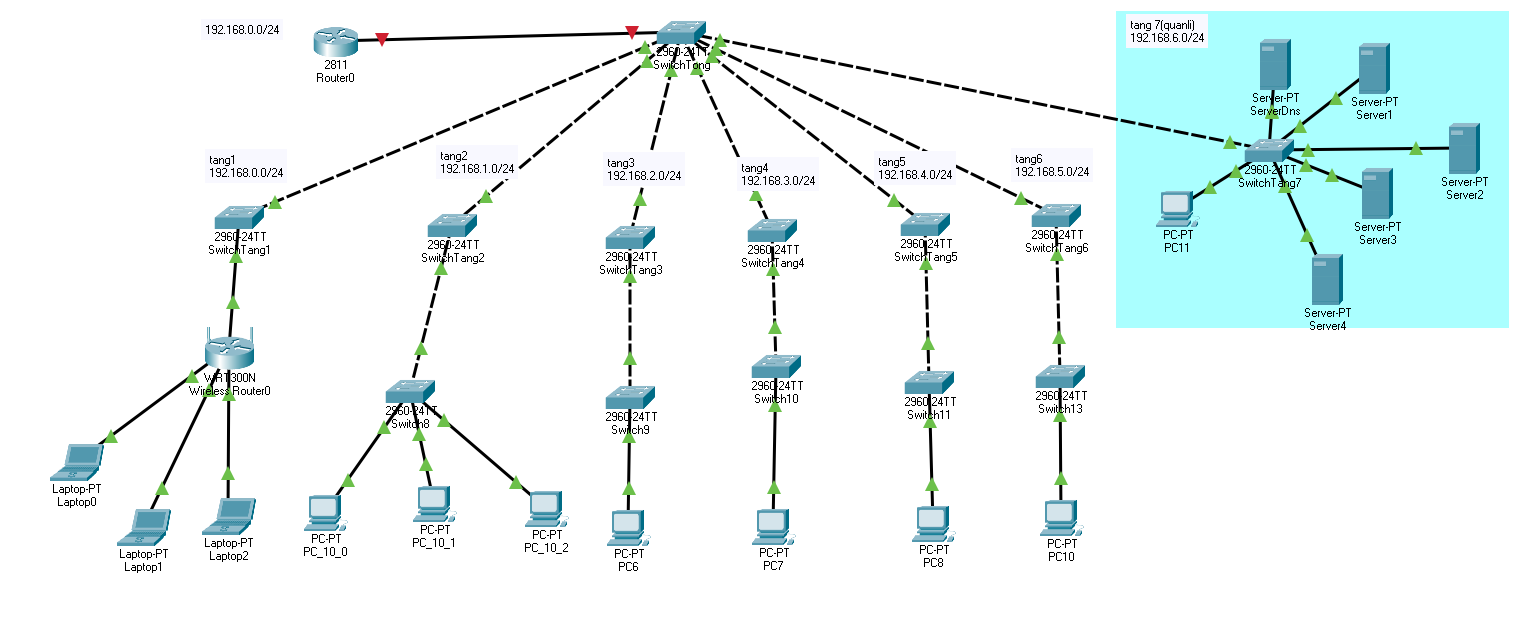
\includegraphics[width=\textwidth]{Images/So_do_logical.png}
    \caption{Sơ đồ luận lý hệ thống mạng tại trụ sở chính}
    \label{fig:So_do_logical}
\end{figure}

\section{Đánh giá hệ thống}
% TODO: Đây chỉ là copied ưu nhược điểm từ bài khác, cần chỉnh lại
\subsection{Ưu điểm}
\begin{itemize}
    \item Mô hình phù hợp với hệ thống mạng lớn.
    \item Dễ dàng quản lý và bảo trì.
    \item Có khả năng mở rộng và nâng cấp.
\end{itemize}
\subsection{Nhược điểm}
\begin{itemize}
    \item Có khả năng hệ thống trì trệ khi server bị hỏng.
    \item Chưa có sự quản lý chặt chẽ trong vấn đề kiểm soát bộ phận cấp nguồn, nếu có sự cố sẽ gây mất hoặc hư hỏng dữ liệu.
    \item Tuy đảm bảo không truy cập được VLAN nội bộ từ bên ngoài, nhưng vẫn không có khả năng chống xâm nhập nếu người khác có chủ ý và sử dụng các công nghệ nâng cao. 
\end{itemize}

%%%%%%%%%%%%%%%%%%%%%%%%%%%%%%%%%%%%%%%%%%%%%%%%%%%%%%%%%
%                   END THIS REPORT                     %
%%%%%%%%%%%%%%%%%%%%%%%%%%%%%%%%%%%%%%%%%%%%%%%%%%%%%%%%%
\newpage
% \addcontentsline{toc}{section}{Tài liệu}
% \bibliographystyle{unsrt}
% \bibliography{ref}
\end{document}
